In this section we compare our performance with other treatments available in the literature in terms of the runtime cost per likelihood evaluation for a single bin.
We perform our tests using a single \texttt{Intel\textsuperscript{\textregistered} Core\texttrademark{} i5-8350U CPU @ 1.70GHz} running code compiled with \texttt{clang version 6.0.0-1ubuntu2}.
We compute the likelihood CPU-evaluation time for the following likelihoods: $\adhoc$, modified-$\chi^2$, $\gl$~\cite{Glusenkamp:2017rlp}, $\lbarlow$~\cite{Barlow:1993dm}, and $\mcl$.
For each of them we consider increasing number of MC events from $10^2$ to $10^6$, increasing number of background components from $1$ to $10^3$, and increasing counts of data events from $10^1$ to $10^4$.
Figure~\ref{fig:performance} shows the behavior of the runtime with respect to these quantities.
All likelihoods have runtime that increases with the number of MC events, as seen in the leftmost panel of Fig.~\ref{fig:performance}, as each likelihood must compute the sum of event weights which incurs an $\mathcal{O}(m)$ cost, where $m$ is the number of MC events in the bin.
Additionally at low MC sample sizes the modified-$\chi^2$ is faster than $\mcl$ since $\mcl$ requires the evaluation of more expensive special functions, however at larger MC sample sizes this additional cost is negligible compared to that of summing the MC weights.
In the middle panel of Fig.~\ref{fig:performance} it can be seen that all likelihoods except $\lbarlow$ are constant with respect to the number of background components as they only depend on summary statistics of the weight distribution.
The Barlow-Beeston likelihood, $\lbarlow$, incurs an $\mathcal{O}(b d \log d)$ cost for solving a single root finding problem per physical component, where $b$ is the number of background components and $d$ is the number of digits of precision, and therefore is not constant in runtime with respect to the number of components.
However, one key difference between $\lbarlow$ and $\mcl$ is that $\mcl$ must compute two summations (the sum of the weights and sum of the square weights), while $\lbarlow$ needs only to compute a single summation of the MC weights.
The rightmost panel of Fig.~\ref{fig:performance} shows the runtime as a function of the number of data events; for most likelihoods the number of data events, $k$, enters only in the evaluation of some special functions which for all practical applications are approximately constant in runtime.
$\gl$ evaluates a special function which for these purposes can only be computed in $\mathcal{O}(k^2 m)$ time, resulting in the dependence on the number of data events.
The $\adhoc$ treatment is always the fastest, but it does not incorporate MC statistical uncertainties in any way.

These tests make the behavior clear for single likelihood evaluations, and we expect similar trends for the runtime when applied to inference problems that are solved using MCMC techniques.
However, additional complications can arise for inference techniques that make use of the profile likelihood.
Global minimization can be affected by the numerical precision of the likelihood evaluation and any discontinuities that result.
We have found such performance issues for $\lbarlow$ and $\gl$, while other techniques seem to have better numerical stability.
While it may be possible to overcome these issues for $\lbarlow$ and $\gl$, currently known techniques have fallen short.

\begin{figure}[ht]
\centering
        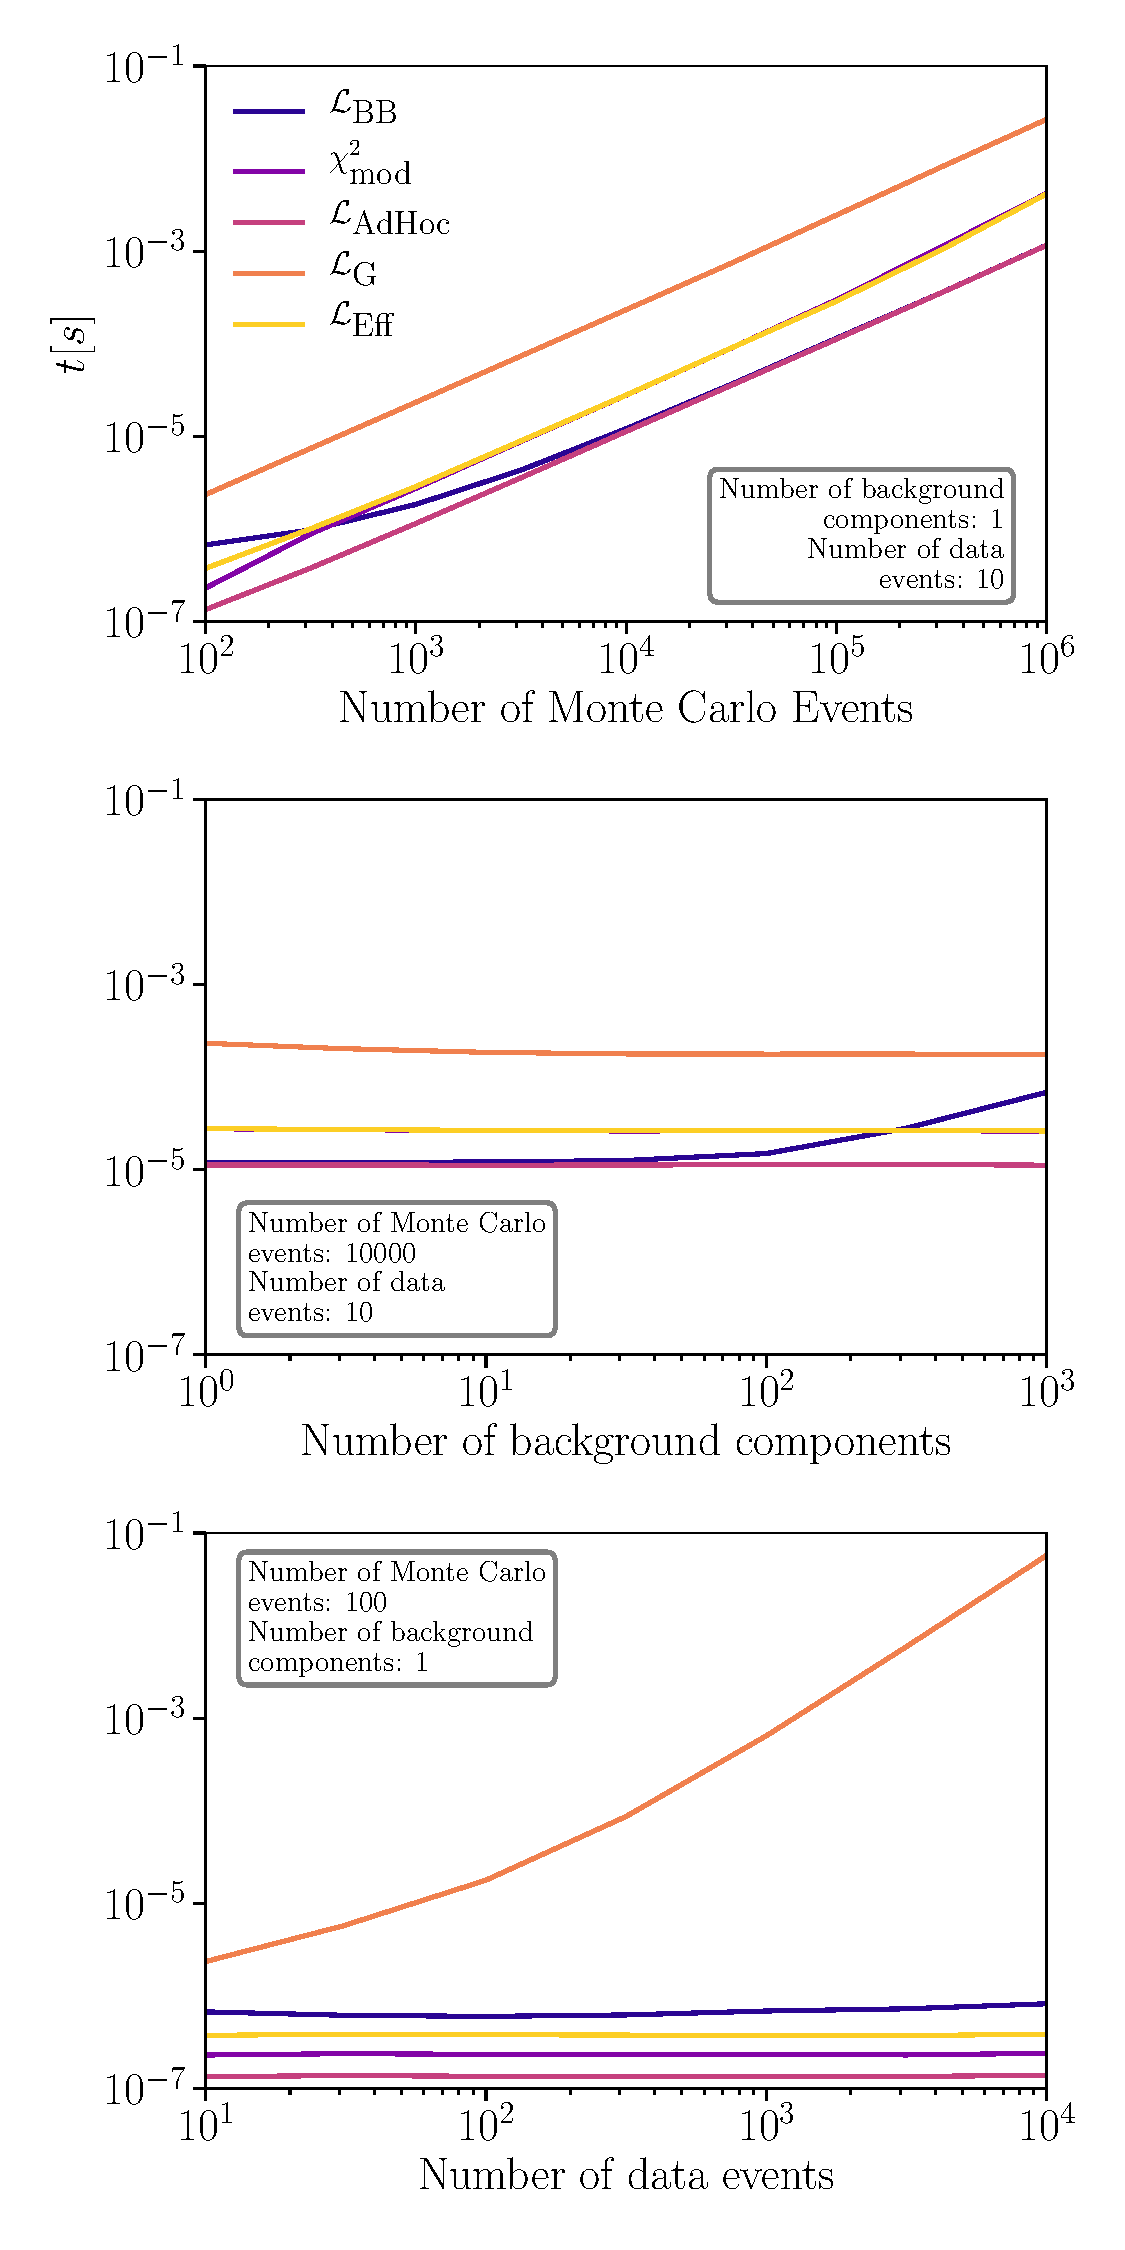
\includegraphics[width=\textwidth,height=0.8\textheight,keepaspectratio]{fig/fig7_multi_panel}
\caption{\textbf{\textit{Likelihood function performance.}} Average single likelihood evaluation time is shown in the vertical axis in seconds.
Different line colors show different likelihoods.
Top-most panel: the number of MC events used is shown on the horizontal axis.
Center panel: the number of background components is shown on the horizontal axis.
Bottom-most panel: the number of data events is show on the horizontal axis.}
\label{fig:performance}
\end{figure}
